\documentclass[conference]{IEEEtran}
\IEEEoverridecommandlockouts
\usepackage{cite}
\usepackage{amsmath,amssymb}
\usepackage{graphicx}
\usepackage{booktabs}
\usepackage{array}
\usepackage{xcolor}
\usepackage{tikz}
\usetikzlibrary{positioning,arrows.meta,fit}
\usepackage[hidelinks]{hyperref}

\newcommand{\NProg}{600}
\newcommand{\NFam}{8}
\newcommand{\NFailed}{0}
\newcommand{\RecAllN}{600}
\newcommand{\RecAllRMS}{1.17}
\newcommand{\RecAllMedRMS}{0.20}
\newcommand{\RecAllIoU}{0.925}
\newcommand{\RecAllHoleRec}{100.0\%}
\newcommand{\RecAllHolePrec}{99.9\%}
\newcommand{\RecAllHoleD}{0.37}
\newcommand{\RecAllHolePos}{0.18}
\newcommand{\RecKnownN}{448}
\newcommand{\RecKnownRMS}{0.19}
\newcommand{\RecKnownMedRMS}{0.11}
\newcommand{\RecKnownIoU}{0.999}
\newcommand{\RecKnownHoleRec}{100.0\%}
\newcommand{\RecKnownHolePrec}{99.8\%}
\newcommand{\RecKnownHoleD}{0.01}
\newcommand{\RecKnownHolePos}{0.18}
\newcommand{\RecInfN}{152}
\newcommand{\RecInfRMS}{4.06}
\newcommand{\RecInfMedRMS}{3.82}
\newcommand{\RecInfIoU}{0.709}
\newcommand{\RecInfHoleRec}{100.0\%}
\newcommand{\RecInfHolePrec}{100.0\%}
\newcommand{\RecInfHoleD}{1.44}
\newcommand{\RecInfHolePos}{0.18}
\newcommand{\RunMean}{1.72}
\newcommand{\RunPNF}{3.92}
\newcommand{\TextRawARI}{0.074}
\newcommand{\TextRawNMI}{0.197}
\newcommand{\TextRawPURITY}{0.232}
\newcommand{\TextRawPATFIVE}{0.558}
\newcommand{\TextRawMAP}{0.205}
\newcommand{\TextCodesARI}{0.055}
\newcommand{\TextCodesNMI}{0.177}
\newcommand{\TextCodesPURITY}{0.230}
\newcommand{\TextCodesPATFIVE}{0.580}
\newcommand{\TextCodesMAP}{0.237}
\newcommand{\ProcARI}{0.572}
\newcommand{\ProcNMI}{0.668}
\newcommand{\ProcPURITY}{0.695}
\newcommand{\ProcPATFIVE}{0.922}
\newcommand{\ProcMAP}{0.746}
\newcommand{\GeoARI}{0.618}
\newcommand{\GeoNMI}{0.720}
\newcommand{\GeoPURITY}{0.777}
\newcommand{\GeoPATFIVE}{0.934}
\newcommand{\GeoMAP}{0.774}
\newcommand{\FullARI}{0.797}
\newcommand{\FullNMI}{0.822}
\newcommand{\FullPURITY}{0.907}
\newcommand{\FullPATFIVE}{0.939}
\newcommand{\FullMAP}{0.851}
\newcommand{\TextRawDialect}{0.609}
\newcommand{\TextCodesDialect}{0.584}
\newcommand{\FullKAuto}{9}
\newcommand{\FullARIAuto}{0.770}
\newcommand{\FullHDBARI}{0.815}
\newcommand{\FullHDBOut}{12.7\%}
\newcommand{\FullHDBK}{10}
\newcommand{\CrossDialectPrec}{94.0\%}
\newcommand{\CrossDialectShare}{74.8\%}
\newcommand{\TINTools}{339}
\newcommand{\TICoverage}{55.5\%}
\newcommand{\TIExact}{43.1\%}
\newcommand{\TIOneSize}{81.9\%}
\newcommand{\DINParts}{40}
\newcommand{\DINProgs}{160}
\newcommand{\DISamePart}{0.921}
\newcommand{\DISameFam}{0.500}
\newcommand{\DIOther}{-0.083}
\newcommand{\DIDesc}{25.0\%}
\newcommand{\ResCoarseRMS}{0.69}
\newcommand{\ResCoarseIoU}{0.961}
\newcommand{\ResCoarseTime}{0.39}
\newcommand{\ResCoarseHoleD}{0.27}
\newcommand{\ResMidRMS}{0.69}
\newcommand{\ResMidIoU}{0.961}
\newcommand{\ResMidTime}{1.75}
\newcommand{\ResMidHoleD}{0.24}
\newcommand{\ResFineRMS}{0.70}
\newcommand{\ResFineIoU}{0.961}
\newcommand{\ResFineTime}{4.95}
\newcommand{\ResFineHoleD}{0.24}
\newcommand{\FeatureRows}{circular pocket & 75 & 1.000 & 0.987 \\
hole & 1542 & 0.999 & 1.000 \\
outline & 319 & 1.000 & 0.962 \\
pocket & 582 & 0.974 & 0.909 \\
pocket island & 75 & 0.904 & 1.000 \\
slot & 262 & 0.834 & 1.000 \\
step & 187 & 0.955 & 0.797 \\}
\newcommand{\HandRows}{\texttt{fanuc\_\allowbreak cutter\_\allowbreak comp} (32 lines) & 4x hole $\varnothing$9, 1x outline \newline \footnotesize{warnings: Controller-side cutter compensation} \\
\texttt{haas\_\allowbreak subprogram} (44 lines) & 4x pocket 20x20x2 \newline \footnotesize{warnings: none} \\
\texttt{helical\_\allowbreak no\_\allowbreak comments} (32 lines) & 4x hole $\varnothing$6, 1x pocket 38x28x3 \newline \footnotesize{warnings: T8} \\
\texttt{lathe\_\allowbreak program} (14 lines) & 1x slot 36x6x25 \newline \footnotesize{warnings: Looks like a lathe; Non-XY plane} \\
\texttt{linuxcnc\_\allowbreak style} (35 lines) & 2x step \newline \footnotesize{warnings: Unsupported code G64 ignored} \\
\texttt{macro\_\allowbreak bolt\_\allowbreak circle} (26 lines) & 1x step \newline \footnotesize{warnings: Macro variables / control flow} \\}


\begin{document}

\title{NC-Archaeologist: Recovering Machined Geometry and Group-Technology Part Families from Legacy CNC Programs}

\author{\IEEEauthorblockN{Sanjit Patibanda}
\IEEEauthorblockA{\textit{School of Mechanical Engineering}\\
\textit{Vellore Institute of Technology}\\
Chennai, India \\
sanjit.patibanda2024@vitstudent.ac.in}}

\maketitle

\begin{abstract}
Machine shops accumulate thousands of CNC part programs whose CAD models have
been lost, leaving archives that cannot be searched, reused or analysed for
Group Technology (GT). We present NC-Archaeologist, a system that works from the
G-code alone. It (i) parses programs across controller dialects, (ii) recovers
the machined part by 2.5D dexel simulation of material removal, (iii) infers
missing cutter diameters from toolpath geometry, (iv) recognises machining
features and builds a process sheet, and (v) forms GT part families from a
rotation-invariant fingerprint of the recovered geometry and process. On a
benchmark of \NProg{} programs from \NFam{} part families written in four
dialects with random fixturing, the recovered parts reach a mean removed-volume
IoU of \RecAllIoU{} against design intent. Family discovery reaches an adjusted
Rand index of \FullARI{} and retrieval reaches precision@5 of \FullPATFIVE{}.
Both are well above text-based baselines (ARI \TextRawARI{}). On \RealN{}
open-source LinuxCNC programs not produced by our generator, \RealAnalysed{} are
analysed, including parametric and macro programs, and recognisable parts are
recovered. To the best of our knowledge, this is the first approach that forms
GT part families directly from subtractive CNC programs.
\end{abstract}

\begin{IEEEkeywords}
computer-integrated manufacturing, G-code, group technology, reverse engineering, dexel simulation, CAPP, part family formation
\end{IEEEkeywords}

%======================================================================
\section{Introduction}
Computer-integrated manufacturing (CIM) rests on the flow of information
between CAD, process planning (CAPP), CAM and the CNC controller~\cite{groover2019,xu2009}.
In practice this flow often runs one way. The NC program is the artefact that
survives on the shop floor, while the CAD model and the planner's intent are
lost when systems are migrated, suppliers change or programmers retire. A shop
may hold thousands of programs named like \texttt{O1234.nc} that nobody can
classify. This blocks three classic CIM benefits:
\begin{itemize}
\item \textbf{Reuse:} recognising that a new part resembles one already
machined, so that a proven program can be adapted;
\item \textbf{Group Technology:} forming part families for cell design and
standardised set-ups~\cite{opitz1970,burbidge1989};
\item \textbf{Digital transformation:} turning an opaque archive into searchable data.
\end{itemize}

Classical GT coding needs a drawing or CAD model, and production-flow analysis
needs route sheets~\cite{burbidge1989}. Neither may exist for legacy parts.
The G-code text itself is a poor basis for comparison. The same part can be
posted with different units, absolute or incremental moves, canned cycles or
explicit pecks, arcs or chords, and any rotation or work offset. Two programs
for one part can therefore share almost no text.

We instead treat each program as an executable description of geometry. We
replay it, recover what it makes, and compare programs by that result. This
paper contributes:
\begin{enumerate}
\item a dialect-tolerant G-code interpreter that also executes parametric
programs (variables, expressions, loops, subroutines, polar coordinates), with
explicit warnings for constructs it cannot execute faithfully (cutter
compensation, external subprograms, lathe code);
\item recovery of the machined part by dexel simulation, including a
\emph{raster-run} heuristic that infers cutter diameters missing from programs
without tool comments, and a stock-footprint estimate from the facing toolpath;
\item multi-level, nesting-aware recognition of holes, pockets, slots, steps
and island pockets on the recovered part, plus an automatically generated process sheet;
\item a rotation- and translation-invariant fingerprint combining recovered
geometry with process content, used for GT family discovery and similarity search;
\item a benchmark of \NProg{} programs in four controller dialects with ground
truth, plus hand-written programs that exercise vendor-specific constructs.
\end{enumerate}

%======================================================================
\section{Related Work}
\textbf{Reverse engineering from toolpaths.} Recovering geometry from G-code has
been studied for \emph{additive} manufacturing. Tsoutsos \emph{et al.}
reconstruct printed solids from toolpaths to detect malicious design changes~\cite{tsoutsos2017}.
Kiński and Sobieski rebuild surfaces from printer G-code through point sets and
Poisson reconstruction, motivated by lost solid models~\cite{kinski2020}. In
additive toolpaths the deposited material \emph{is} the part. In milling the
part is what \emph{remains} after the cutter has removed material. So the
reverse problem requires simulating removal with the correct cutter geometry,
which these methods do not address.

\textbf{Group Technology and part families.} GT classification uses coding
systems such as Opitz~\cite{opitz1970}, production-flow analysis~\cite{burbidge1989},
and a large literature on cell-formation algorithms~\cite{selim1998,kusiak1987}.
All of these assume design attributes or routing data as input.

\textbf{Feature recognition and plan reuse.} Machining-feature recognition from
B-rep solids is mature~\cite{han2000}, and CAD-model retrieval has been used to
reuse process plans~\cite{pitta2005}. Both require the CAD model, which is
exactly what is missing for legacy programs.

\textbf{Learning on G-code.} Recent work uses large language models to
\emph{generate} G-code~\cite{abdelaal2025}, and notes that G-code carries no
semantic description of the geometry it produces. We address the inverse
problem: recovering that geometry and using it.

\textbf{Simulation.} The dexel (depth-element) representation for NC
verification goes back to van Hook~\cite{vanhook1986}. We use its height-map
form as a fast, adequate model for 3-axis prismatic parts.

%======================================================================
\section{Method}
Fig.~\ref{fig:arch} shows the pipeline.

\begin{figure}[t]
\centering
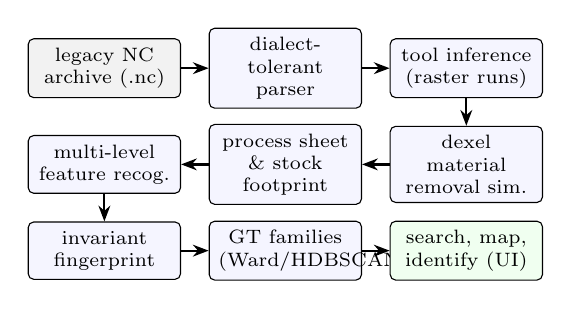
\begin{tikzpicture}[
  box/.style={draw, rounded corners=2pt, align=center, font=\scriptsize, minimum height=7mm, text width=17mm, fill=blue!4},
  arr/.style={-{Stealth[length=2mm]}, thick}, node distance=3.5mm]
\node[box, fill=gray!10] (in) {legacy NC\\archive (.nc)};
\node[box, right=of in] (p) {dialect-tolerant\\parser};
\node[box, right=of p] (t) {tool inference\\(raster runs)};
\node[box, below=of t] (s) {dexel material\\removal sim.};
\node[box, left=of s] (pr) {process sheet\\\& stock footprint};
\node[box, left=of pr] (fr) {multi-level\\feature recog.};
\node[box, below=of fr] (fp) {invariant\\fingerprint};
\node[box, right=of fp] (gt) {GT families\\(Ward/HDBSCAN)};
\node[box, right=of gt, fill=green!6] (ui) {search, map,\\identify (UI)};
\draw[arr] (in) -- (p); \draw[arr] (p) -- (t); \draw[arr] (t) -- (s);
\draw[arr] (s) -- (pr); \draw[arr] (pr) -- (fr); \draw[arr] (fr) -- (fp);
\draw[arr] (fp) -- (gt); \draw[arr] (gt) -- (ui);
\end{tikzpicture}
\caption{NC-Archaeologist pipeline. Only the G-code is used as input.}
\label{fig:arch}
\end{figure}

\subsection{Dialect-tolerant interpretation}
A tokenizer and modal state machine follow ISO~6983~\cite{iso6983}. They handle
motion modes G0--G3 (IJK and R arcs, helical moves), units G20/G21, distance
modes G90/G91, canned drilling cycles G81--G83 with G98/G99 retract, tool
changes and work offsets. Arcs are linearised to a 0.05\,mm chord tolerance.
Fanuc subprograms (\texttt{M98}/\texttt{O}\,\dots\,\texttt{M99}) defined in
the same file are inlined. Parametric programs are executed by a macro layer
before interpretation: numbered and named parameters, bracket expressions with
arithmetic, comparison and trigonometric functions, LinuxCNC \texttt{o}-word
subroutines with arguments, \texttt{if}/\texttt{while}/\texttt{repeat}, and
Fanuc Macro~B \texttt{WHILE\dots DO}/\texttt{END} and \texttt{IF\dots GOTO}.
Polar coordinates (\texttt{@} radius, \texttt{\^{}} angle) and repeat counts
\texttt{L} on canned cycles are supported. Constructs the interpreter cannot
execute faithfully are \emph{flagged rather than guessed}: controller-side
cutter compensation G41/G42, calls to subprograms in other files, non-XY
planes, several work offsets in one program (fixture stations drawn in one
frame) and lathe programs. Each program carries these warnings into the user
interface.

\subsection{Cutter inference}
Diameters are read from tool comments when present. Many legacy programs have
no comments, so we infer the diameter from geometry. Inside a \emph{raster run}
(at least three alternating, parallel, equal-$Z$ passes joined by short link
moves with no rapid in between), the pass spacing equals the step-over $s$.
Requiring this pattern rejects look-alikes such as separate parallel slots or
the two long sides of a profile loop. With a typical step-over ratio of 0.5,
$\hat D = \mathrm{snap}(s/0.5)$ to the nearest standard cutter. A single
shallow level of long passes is treated as facing, with ratio 0.7. Drills and
non-raster tools fall back to a default diameter, and the program is flagged.

\subsection{Material-removal simulation}
The stock is a height map $Z_{ij}$ (default 0.25\,mm cells) over the XY
extent of all cutting moves. The stock top is $Z{=}0$, the most common
convention. Each feed move lowers $Z$ by the swept cutter envelope:
\begin{equation}
Z_{ij} \leftarrow \min\!\big(Z_{ij},\ z(t^\ast) + h(r_{ij})\big),
\end{equation}
where $h$ is the cutter profile (flat, ball, 118$^\circ$ drill point, or
chamfer). For flat cutters the minimum over the move is evaluated in closed
form, using the end points of the covered parameter interval. Shaped cutters
are sampled along the move. Per-tool-block removal masks feed the process analysis.

\subsection{Process sheet and stock footprint}
The program is split into tool blocks. Each block is classified from what it
removed as facing, pocketing, island pocketing, bore, slotting, step milling,
profiling or drilling. The rules use depth, coverage, enclosure (filled-hole
area relative to cut area), elongation relative to cutter width, and contact
with the stock edge. Cycle time is estimated from feed rates, rapid traverse,
tool changes and pecks. G-code does not state the stock size, so we estimate
the stock footprint from the facing toolpath. Facing passes overrun the stock
by about one cutter radius at their ends and overhang the side edges by about
half a radius, so the pass envelope is contracted along and grown across the
passes accordingly.

\subsection{Multi-level feature recognition}
Flat-floor depths (cells with near-zero slope, so drill cones and scallops are
ignored) define plateau levels. Connected regions are extracted between
successive levels after morphological smoothing. Each region becomes a feature
whose parent is the region containing it one level up, and a region identical
to its parent is not repeated. Regions are labelled as hole, circular pocket,
pocket, slot, step, island pocket or outline. The labels use circularity, a
fill ratio that separates circles (about 0.785) from rounded squares (about 1),
principal-axis aspect ratio, enclosed uncut area and stock-edge contact. Hole
patterns are tested for a common pitch circle diameter.

\subsection{Fingerprint and family discovery}
A fingerprint should describe \emph{what} a program makes, independent of
how it is written or fixtured. The geometric block is computed on a
design-depth image from which facing, the outer profiling ring and cuts in air
outside the estimated stock are removed. It contains the depth histogram
relative to the deepest cut, the seven Hu moment invariants~\cite{hu1962},
a radial depth profile normalised by the radius of gyration, log feature
counts, elongation, normalised hole size, bolt-circle flag and nesting. All of
these are invariant to rotation and translation. The process block contains
the operation-time mix, operation presence and counts, and tool statistics.
Each block is standardised, weighted (0.5/0.5, chosen on a separate
development set) and normalised by its dimension. Families come from Ward
agglomerative clustering~\cite{ward1963}, with $k$ chosen by silhouette when
unknown. HDBSCAN~\cite{campello2013} provides density-based families and flags
unusual programs. Similarity search uses cosine $k$-NN, and the archive map
uses t-SNE~\cite{vandermaaten2008}.

\subsection{Implementation and interactive dashboard}
The system is written in Python (about 3,800 lines, using NumPy, SciPy,
scikit-image and scikit-learn) with 22 unit tests for the interpreter, the
macro layer and the simulator. A FastAPI back end serves a browser dashboard (Fig.~\ref{fig:dash})
built with Three.js and Plotly. Users can browse the archive map and the
discovered families, inspect a recovered part in 3D, and replay its machining:
the replay lowers the height map move by move and shows the G-code line being
executed. The dashboard also shows the process sheet, recognised features and
similar programs, and explains every G-code line in plain language. Any new
program can be uploaded and is analysed and assigned to a family in about two
seconds, which makes the method usable as an everyday archive tool rather than
an offline experiment.

\begin{figure*}[t]
\centering
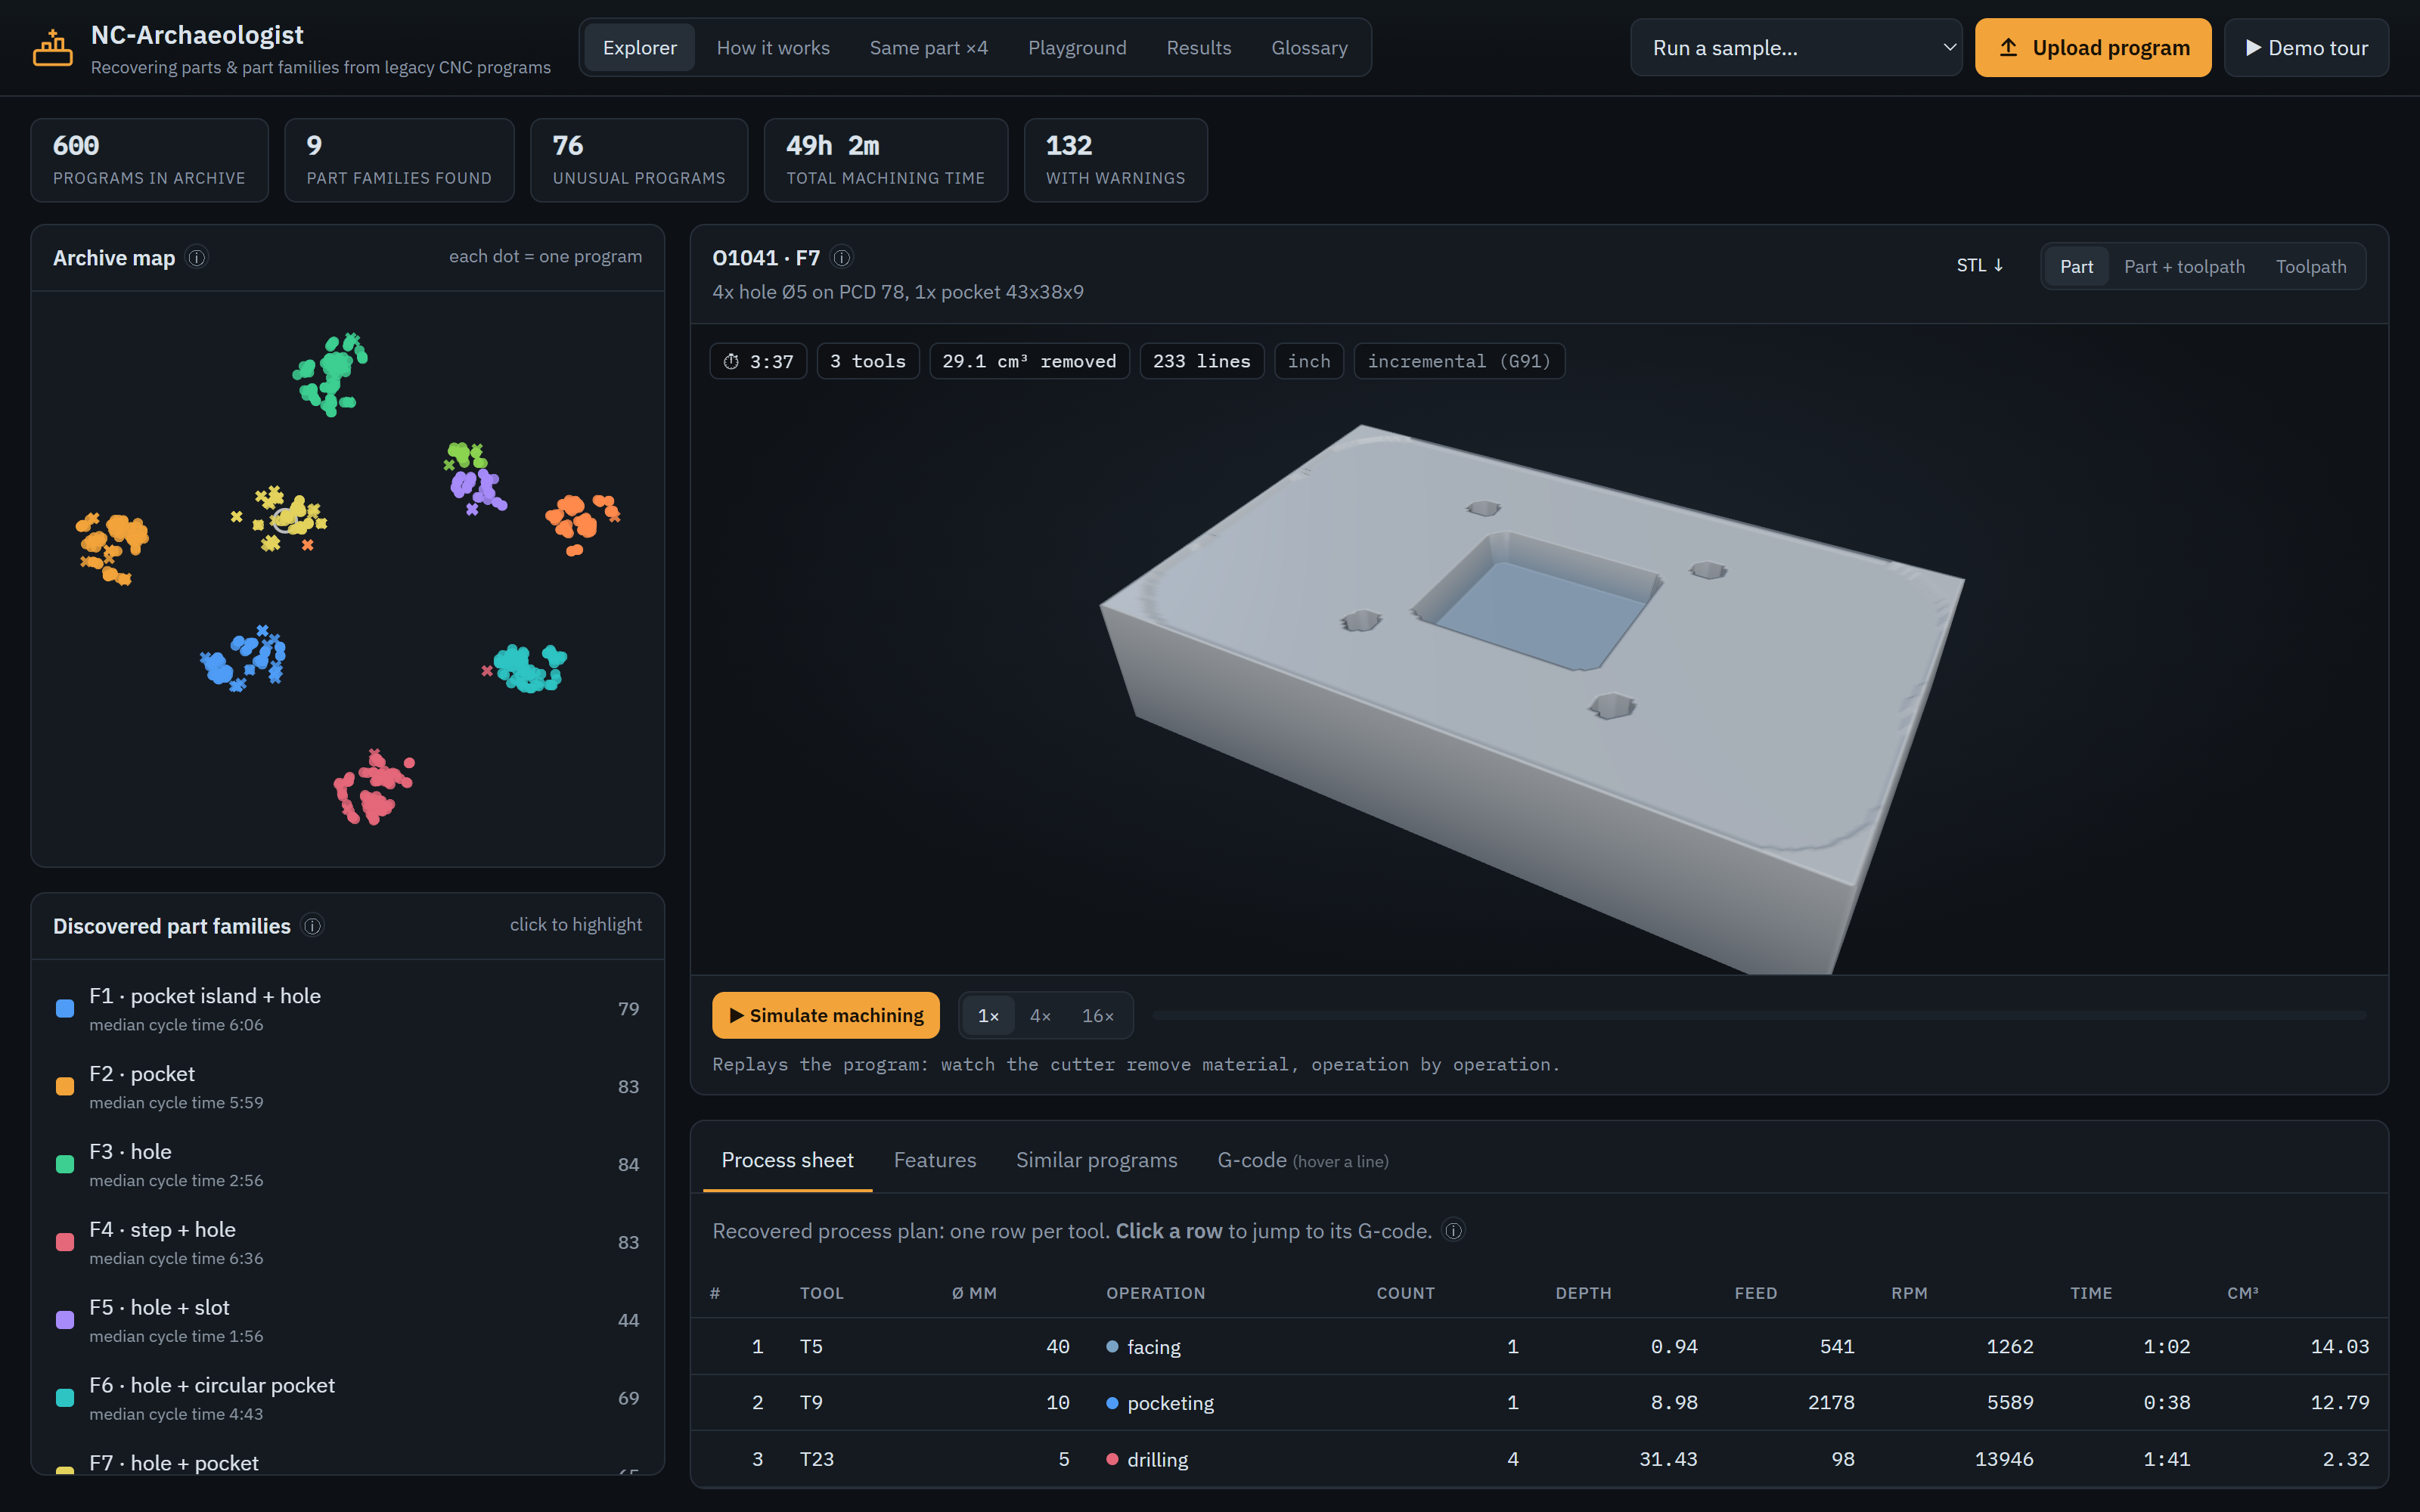
\includegraphics[width=\textwidth]{figs/dashboard.png}
\caption{NC-Archaeologist dashboard on the 600-program test archive: fingerprint map coloured by discovered family (left), automatically named families, a part recovered from an inch/incremental program with machining replay, and its recovered process sheet.}
\label{fig:dash}
\end{figure*}

%======================================================================
\section{Benchmark}
No public archive of CNC programs with part-family labels exists, so we built
a synthetic benchmark with a fully known ground truth. We state this openly and
complement it with hand-written programs (Section~\ref{sec:hand}).
\begin{itemize}
\item \textbf{Eight parametric families}: bolt-hole plate, pocket housing,
slotted bracket, flange, stepped block, multi-pocket tray, keyway bar and boss
(island in pocket). Dimensions, counts, depths, cutters and optional facing
and profiling are randomised.
\item \textbf{A mini CAM}: zig-zag or offset-spiral pocketing, concentric
bores, multi-level slots, shoulder rasters, peck or canned drilling, and
climb or conventional profiles. Step-over is 40--60\,\% and step-down 1.5--3.5\,mm.
\item \textbf{Four post-processor dialects}: Fanuc-like with N-numbers, IJ arcs
and G83; Haas-like with R arcs and G81/G83 cycles; \emph{minimal} with no
comments, chord-linearised arcs and explicit pecks; and inch + incremental
(G20/G91).
\item \textbf{Random fixturing}: rotation (half at 0$^\circ$, a quarter at
multiples of 90$^\circ$, a quarter arbitrary) and work zero at the stock
centre or corner.
\end{itemize}
File names carry no family information. Ground truth (family, design spec and
an analytic design-depth function) is used only for evaluation. All parameters
were tuned on a development set (seed 7). All reported results are on a
held-out test set of \NProg{} programs (seed 11, 75 per family).

%======================================================================
\section{Results}
\subsection{Part recovery}
Table~\ref{tab:recon} compares recovered depth maps with the analytic design
intent inside the physical stock. Programs whose tools are all named in
comments are recovered almost exactly. Programs that rely on inferred or
default cutters (all from the comment-free dialect) lose accuracy wherever a
diameter falls back to the default: drills, single-pass slots and profile
passes. The skewed distribution (mean vs.\ median RMS) reflects these cases. Hole positions are recovered to within
\RecAllHolePos{}\,mm on average. Mean runtime is \RunMean{}\,s per program
(95th percentile \RunPNF{}\,s) on a laptop CPU.

\begin{table}[t]
\caption{Recovered part vs.\ design intent (test set)}
\label{tab:recon}
\centering\footnotesize
\begin{tabular}{lccc}
\toprule
 & all & tools in comments & tools inferred \\
\midrule
programs & \RecAllN & \RecKnownN & \RecInfN \\
removed-volume IoU & \RecAllIoU & \RecKnownIoU & \RecInfIoU \\
RMS depth error (mm) & \RecAllRMS & \RecKnownRMS & \RecInfRMS \\
median RMS (mm) & \RecAllMedRMS & \RecKnownMedRMS & \RecInfMedRMS \\
hole recall & \RecAllHoleRec & \RecKnownHoleRec & \RecInfHoleRec \\
hole precision & \RecAllHolePrec & \RecKnownHolePrec & \RecInfHolePrec \\
hole $\varnothing$ MAE (mm) & \RecAllHoleD & \RecKnownHoleD & \RecInfHoleD \\
\bottomrule
\end{tabular}
\end{table}

Table~\ref{tab:feat} reports count-based precision and recall of feature
recognition per type. Fig.~\ref{fig:pipeline} shows an example.

\begin{table}[t]
\caption{Feature recognition (count-matched, test set)}
\label{tab:feat}
\centering\footnotesize
\begin{tabular}{lccc}
\toprule
feature & \# in ground truth & precision & recall \\
\midrule
\FeatureRows
\bottomrule
\end{tabular}
\end{table}

\begin{figure*}[t]
\centering
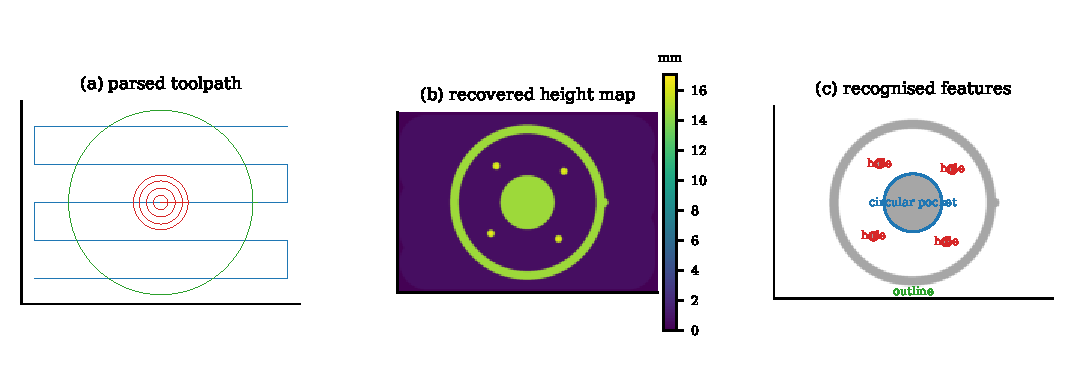
\includegraphics[width=\textwidth]{figs/pipeline.pdf}
\caption{A flange program (Haas dialect): (a) parsed toolpath, (b) recovered height map, (c) recognised features and bolt circle.}
\label{fig:pipeline}
\end{figure*}

\begin{figure*}[t]
\centering
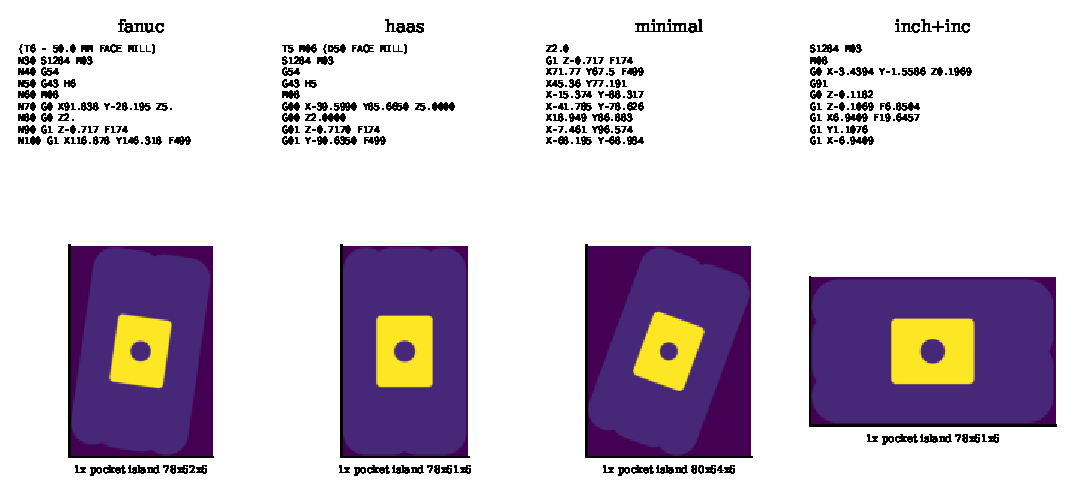
\includegraphics[width=\textwidth]{figs/dialects.pdf}
\caption{One part posted in four dialects with independent fixturing. The text differs completely, while the recovered parts and recognised features agree.}
\label{fig:dialects}
\end{figure*}

\subsection{Cutter inference}
On the comment-free dialect, raster-run inference covered \TICoverage{} of
the \TINTools{} milling tools. Of these, \TIExact{} were identified exactly
and \TIOneSize{} were within one standard size. The remainder (single-pass
slots, spiral-only pockets and profiles) fell back to the default diameter and
were flagged to the user.

\subsection{Part-family discovery and retrieval}
Table~\ref{tab:fam} and Fig.~\ref{fig:ablation} compare the full fingerprint
with four baselines. Text TF-IDF works either on raw character $n$-grams or on
the sequence of G/M/T codes with coordinates removed. The process-only and
geometry-only variants use one block of our fingerprint each. Text baselines
mostly recover the posting \emph{dialect} rather than the part family: their
clusters agree with the dialect labels at ARI \TextRawDialect{} (raw) and
\TextCodesDialect{} (codes), but with the true families at only \TextRawARI{}
and \TextCodesARI{}.
Combining recovered geometry with process content gives the best results.
Without knowing $k$, the silhouette criterion selects $k{=}\FullKAuto{}$
(ARI \FullARIAuto{}). HDBSCAN finds \FullHDBK{} dense families (ARI
\FullHDBARI{} on inliers) and sets aside \FullHDBOut{} of programs as unusual.

\begin{table}[t]
\caption{Family discovery ($k{=}8$, Ward) and retrieval}
\label{tab:fam}
\centering\footnotesize
\setlength{\tabcolsep}{4pt}
\begin{tabular}{lccccc}
\toprule
representation & ARI & NMI & purity & P@5 & mAP \\
\midrule
text TF-IDF (raw) & \TextRawARI & \TextRawNMI & \TextRawPURITY & \TextRawPATFIVE & \TextRawMAP \\
text TF-IDF (codes) & \TextCodesARI & \TextCodesNMI & \TextCodesPURITY & \TextCodesPATFIVE & \TextCodesMAP \\
process only & \ProcARI & \ProcNMI & \ProcPURITY & \ProcPATFIVE & \ProcMAP \\
geometry only & \GeoARI & \GeoNMI & \GeoPURITY & \GeoPATFIVE & \GeoMAP \\
\textbf{full (ours)} & \textbf{\FullARI} & \textbf{\FullNMI} & \textbf{\FullPURITY} & \textbf{\FullPATFIVE} & \textbf{\FullMAP} \\
\bottomrule
\end{tabular}
\end{table}

\begin{figure}[t]
\centering
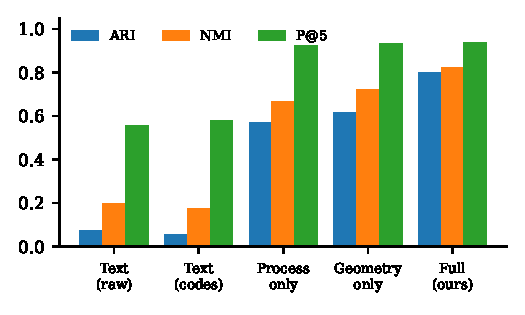
\includegraphics[width=\columnwidth]{figs/ablation.pdf}
\caption{Ablation: clustering (ARI, NMI) and retrieval (P@5).}
\label{fig:ablation}
\end{figure}

\begin{figure}[t]
\centering
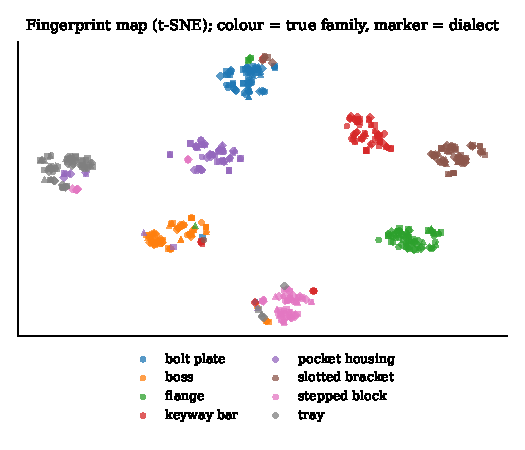
\includegraphics[width=\columnwidth]{figs/tsne.pdf}
\caption{t-SNE map of fingerprints. Colours are true families and markers are
dialects. Dialects mix within each family.}
\label{fig:tsne}
\end{figure}

\begin{figure}[t]
\centering
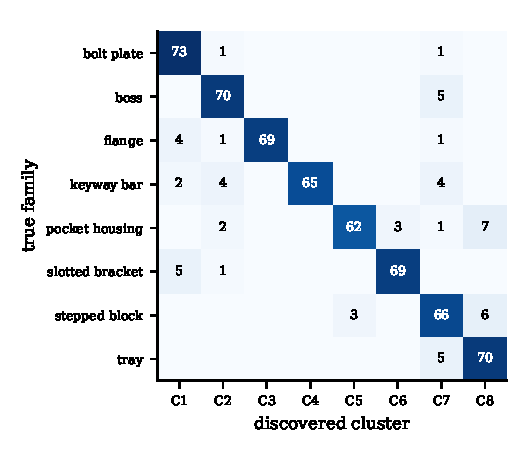
\includegraphics[width=\columnwidth]{figs/confusion.pdf}
\caption{True families vs.\ discovered clusters (Hungarian-matched).}
\label{fig:conf}
\end{figure}

\subsection{Dialect invariance}
Of the top-5 neighbours, \CrossDialectShare{} come from a \emph{different}
dialect than the query, and \CrossDialectPrec{} of those belong to the correct
family (Fig.~\ref{fig:tsne}). In a controlled test, each of \DINParts{} parts
was posted in all four dialects with independent fixturing (\DINProgs{}
programs). The mean cosine similarity between versions of the \emph{same part}
was \DISamePart{}, against \DISameFam{} for different parts of the same family
and \DIOther{} across families. The textual feature descriptions were
character-identical across all four dialects for \DIDesc{} of parts. The
remaining differences are in dimensional detail, chiefly drill diameters that
the comment-free dialect cannot state and 1--2\,mm differences in reported
pocket extents, while feature types and counts agree (Fig.~\ref{fig:dialects}).


\subsection{Resolution trade-off}
On a random sample of 48 programs, the RMS depth error is \ResCoarseRMS{},
\ResMidRMS{} and \ResFineRMS{}\,mm at 0.5, 0.25 and 0.1\,mm cells, while
runtime grows from \ResCoarseTime{} to \ResMidTime{} and \ResFineTime{}\,s
per program. The error is therefore dominated by
modelling factors (cutter inference, stock estimate) rather than by grid
size. Hole diameter error falls slightly with finer cells (\ResCoarseHoleD{}
to \ResFineHoleD{}\,mm). We keep 0.25\,mm as a compromise for feature
measurement; 0.5\,mm would suffice for family discovery alone.


\subsection{Hand-written programs}\label{sec:hand}
Table~\ref{tab:hand} lists hand-written programs that were not produced by our
generator. They exercise vendor constructs: cutter compensation, a Haas
subprogram, a Fanuc Macro~B bolt circle, a helical entry without tool
comments, LinuxCNC o-word subroutines, and a lathe program. The subprogram
and the Macro~B loop are executed and recovered correctly (six holes on the
programmed 80\,mm pitch circle), and cutter compensation and the lathe program
are flagged. One result is wrong in an instructive way: without a facing pass
the stock edge is unknown, so the two LinuxCNC window pockets, which lie at the
edge of the machined area, are labelled as steps.

\subsection{Open-source real programs}\label{sec:real}
To check the interpreter beyond our own generator, we ran \RealN{} programs from
the \texttt{nc\_files} folder of the LinuxCNC project (GPL-2.0), selected as all
3-axis milling examples plus one lathe program, unmodified. They include a
3D carving written entirely with named parameters (4{,}700 lines), a
stepper-motor mount from a workshop machine using macros and three fixture
stations, bolt circles in polar coordinates, cutter-compensation demonstrations
and an interpreter torture test. \RealAnalysed{} programs are analysed; the
other two are not part programs (a remap subroutine and an empty template) and
are correctly rejected for having no cutting moves. The macro layer is needed
in \RealMacro{} of them. These files have no ground truth, so
Table~\ref{tab:real} compares the result with what each file's own comments
say it makes. Hole counts and pitch circles match the comments exactly (26
holes in \texttt{polar}; six holes on PCD 76\,mm for a programmed 3-inch
circle), and the carving and motor mount are recognisable
(Fig.~\ref{fig:real}). Drill and cutter sizes are rarely stated in these
files, so the default diameter is used and flagged, which limits dimensional
accuracy.

\begin{figure}[t]
\centering
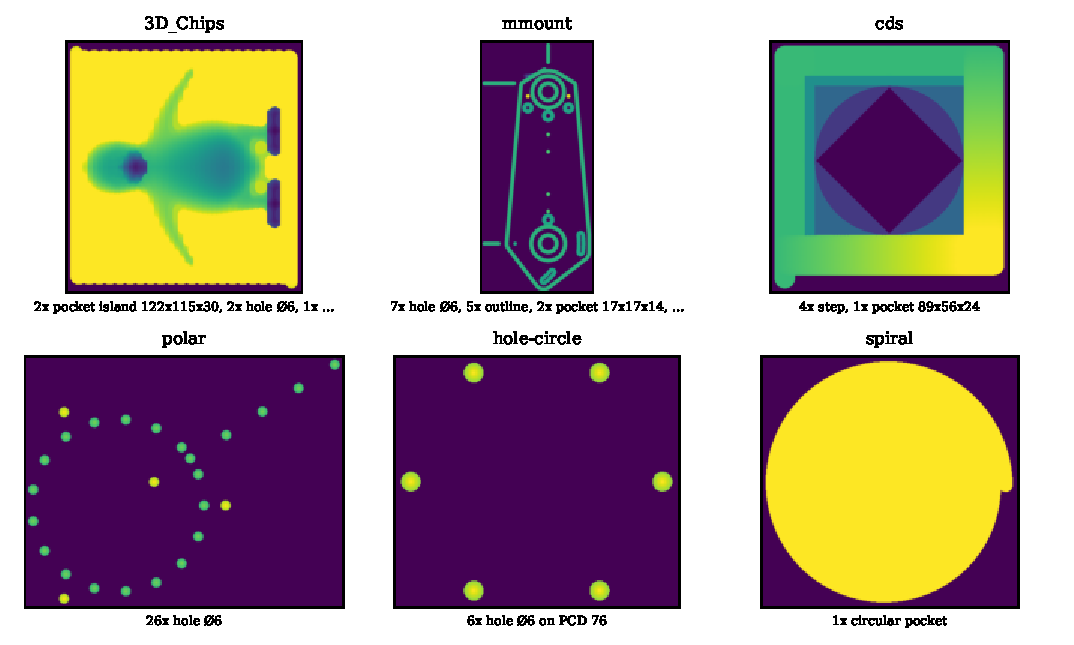
\includegraphics[width=\columnwidth]{figs/real_world.pdf}
\caption{Parts recovered from unmodified LinuxCNC example programs (depth maps, darker = higher).}
\label{fig:real}
\end{figure}

\begin{table}[t]
\caption{Open-source LinuxCNC programs (selected)}
\label{tab:real}
\centering\scriptsize
\begin{tabular}{>{\raggedright}p{1.35cm}>{\raggedright}p{2.75cm}>{\raggedright\arraybackslash}p{3.6cm}}
\toprule
program & stated in the file & recovered \\
\midrule
\RealRows
\bottomrule
\end{tabular}
\end{table}

\begin{table}[t]
\caption{Hand-written test programs (qualitative)}
\label{tab:hand}
\centering\scriptsize
\begin{tabular}{>{\raggedright}p{2.3cm}>{\raggedright\arraybackslash}p{5.6cm}}
\toprule
program & recovered description and warnings \\
\midrule
\HandRows
\bottomrule
\end{tabular}
\end{table}

%======================================================================
\section{Discussion and Limitations}
\begin{itemize}
\item \textbf{Synthetic benchmark.} Families, CAM strategies and dialects were
designed by us. The dialect variety and fixturing randomisation make text
matching fail, but real archives contain more diverse strategies (adaptive
clearing, trochoidal slots). The open-source programs of
Section~\ref{sec:real} show that the interpreter and reconstruction carry over
to real files, but they have no family labels. Quantitative validation on a
labelled shop archive is the most important next step.
\item \textbf{2.5D model.} Height maps cannot represent undercuts, and the
system targets 3-axis prismatic parts.
\item \textbf{Unknown stock and cutters.} Stock size is inferred from facing
when present. Drill diameters cannot be inferred from geometry. Cutter
compensation is flagged rather than resolved.
\item \textbf{Not executed.} Subprograms stored in other files, system
parameters of a specific controller and cutter compensation are flagged rather
than executed. A program using several work offsets is drawn in one frame.
\end{itemize}

\section{Future Work}
Natural extensions are STEP-NC (ISO~14649~\cite{iso14649}) export of the
recovered features, so that legacy parts re-enter a modern CAD/CAPP/CAM chain;
5-axis toolpaths with tri-dexel models; learned fingerprints trained on larger
archives; and linking families to cell formation and shop-floor scheduling.

\section{Conclusion}
NC-Archaeologist shows that a legacy CNC program contains enough information
to recover its part, plan and family. By comparing programs on what they
\emph{make} rather than how they are \emph{written}, it groups parts across
controller dialects and fixturing, a setting where text similarity fails. This
offers a practical route to Group Technology and reuse for shops whose only
record of a part is its G-code.

\begin{thebibliography}{00}
\bibitem{groover2019} M.~P. Groover, \emph{Automation, Production Systems, and Computer-Integrated Manufacturing}, 5th~ed. Pearson, 2019.
\bibitem{xu2009} X.~Xu, \emph{Integrating Advanced Computer-Aided Design, Manufacturing, and Numerical Control: Principles and Implementations}. Hershey, PA: IGI Global, 2009.
\bibitem{opitz1970} H.~Opitz, \emph{A Classification System to Describe Workpieces}. Oxford: Pergamon Press, 1970.
\bibitem{burbidge1989} J.~L. Burbidge, \emph{Production Flow Analysis for Planning Group Technology}. Oxford: Clarendon Press, 1989.
\bibitem{selim1998} H.~M. Selim, R.~G. Askin, and A.~J. Vakharia, ``Cell formation in group technology: review, evaluation and directions for future research,'' \emph{Computers \& Industrial Engineering}, vol.~34, no.~1, pp.~3--20, 1998.
\bibitem{kusiak1987} A.~Kusiak, ``The generalized group technology concept,'' \emph{International Journal of Production Research}, vol.~25, no.~4, pp.~561--569, 1987.
\bibitem{tsoutsos2017} N.~G. Tsoutsos, H.~Gamil, and M.~Maniatakos, ``Secure 3D printing: Reconstructing and validating solid geometries using toolpath reverse engineering,'' in \emph{Proc. 3rd ACM Workshop on Cyber-Physical System Security (CPSS)}, 2017.
\bibitem{kinski2020} W.~Kiński and W.~Sobieski, ``Geometry extraction from GCODE files destined for 3D printers,'' \emph{Technical Sciences}, vol.~23, no.~2, pp.~115--130, 2020, doi: 10.31648/ts.5644.
\bibitem{han2000} J.~Han, M.~Pratt, and W.~C. Regli, ``Manufacturing feature recognition from solid models: a status report,'' \emph{IEEE Trans. Robotics and Automation}, vol.~16, no.~6, pp.~782--796, 2000.
\bibitem{pitta2005} C.~Pitta and M.~M. Marefat, ``Intelligent retrieval and reuse of CAD solid models,'' in \emph{Proc. IEEE Int. Conf. Robotics and Automation (ICRA)}, 2005.
\bibitem{abdelaal2025} M.~Abdelaal, S.~Lokadjaja, and G.~Engert, ``GLLM: Self-corrective G-code generation using large language models with user feedback,'' in \emph{Proc. BTW 2025 (Industrial Track)}, 2025, arXiv:2501.17584.
\bibitem{vanhook1986} T.~Van~Hook, ``Real-time shaded NC milling display,'' \emph{ACM SIGGRAPH Computer Graphics}, vol.~20, no.~4, pp.~15--20, 1986.
\bibitem{iso6983} ISO 6983-1:2009, \emph{Automation systems and integration --- Numerical control of machines --- Program format and definitions of address words}.
\bibitem{iso14649} ISO 14649-1:2003, \emph{Industrial automation systems and integration --- Physical device control --- Data model for computerized numerical controllers}.
\bibitem{hu1962} M.-K. Hu, ``Visual pattern recognition by moment invariants,'' \emph{IRE Trans. Information Theory}, vol.~8, no.~2, pp.~179--187, 1962.
\bibitem{ward1963} J.~H. Ward, ``Hierarchical grouping to optimize an objective function,'' \emph{J. American Statistical Association}, vol.~58, no.~301, pp.~236--244, 1963.
\bibitem{campello2013} R.~J. G.~B. Campello, D.~Moulavi, and J.~Sander, ``Density-based clustering based on hierarchical density estimates,'' in \emph{Proc. PAKDD}, LNCS 7819, 2013, pp.~160--172.
\bibitem{vandermaaten2008} L.~van~der~Maaten and G.~Hinton, ``Visualizing data using t-SNE,'' \emph{J. Machine Learning Research}, vol.~9, pp.~2579--2605, 2008.
\end{thebibliography}

\end{document}
